\chapter{Results}

We evaluate the \dBCM based on how well it can identify true \kmer{s} in the unprocessed reads (Section~\ref{sec:results-dbcm-counting}), as well as on how it can further filter out spurious \kmer{s} through traversal of the graph (Section~\ref{sec:results-dbcm-traversal}). We then evaluate how the false positive rate is affected when traversing the \dBHT built from the traversal of the \dBCM (Section~\ref{sec:results-dbht}). All the experiments described herein were carried out with synthetic reads generated using the \emph{ART Illumina} simulation toolkit \cite{Huang2011} of the \emph{E.~Coli} chromosomal DNA \cite{ecoligenome}\paguso{coloca o site de onde tu fez o download} with coverage $c = 80\times$ \paguso{resulting in approximately XXX reads with average length YYY}. The experiments were conducted on a Dell XPS 15 9575, with a $4.1$GHz Intel Core i7-80705G CPU and $16$GB of RAM, plus $8$GB of SSD swap.

We show that exact counts are not needed to filter out the majority of spurious \kmer{s} from the reads, such that a \dBCM using $120$MB of memory can still filter over $80\%$ of the erroneous \kmer{s}, leaving only twice as many as if the exact counts had been used\toconsider{, for which approximately $500$MB of memory would have been required}. Furthermore, traversing the \dBCM and considering only the visited nodes as true \kmer{s} causes the number of false positives to decrease by over $98\%$. Finally, a \dBHT constructed from all the nodes and edges found during traversal of the \dBCM can still be succesfully traversed, with an increase in the number of false \kmer{s} by a factor of $2$, but still keeping the percentage of false nodes on the graph below $5\%$ with a load factor $\alpha = 0.5$, and even with $\alpha = 0.9$ only around $15\%$ of the nodes visited during traversal represented \kmer{s} not found in the original sequence. It also incurs in no loss of sensitivity, with over $99\%$ of true \kmer{s} being represented in the resulting \dBG. 
\paguso{Quase certeza que o avaliador vai dizer que falta uma comparação com outras alternativas pra dizer se isso é bom ou ruim}

\section{The \dBCM as a \dBG representation}
\label{sec:results-dbcm-counting}

To assess how well the \dBCM can represent a \dBG when constructed from the raw sequencing reads, we first analyze how accurately it performs \kmer counting. We constructed a set of \dBCM instances with varying dimensions $w \in \{7.5\text{M}, 10\text{M}, \ldots 17.5\text{M}, 20\text{M}\}$\footnote{$1\mega = 10^6$} and $d \in \{6, 8\}$ from the set of synthetic reads of the \emph{E.~Coli} genome. For each instance, we calculated the $80$, $90$, $95$, and $99$ percentiles of the individual count errors $\Delta(X) = C.\mathit{query}(X) - c(X)$. In Figure~\ref{fig:ecoli-art-dbcm-errors} we plot these metrics as a function of $w$ for the two values of $d$.

\begin{figure}[htb]
    \centering
    \begin{subfigure}{.5\textwidth}
        \centering
        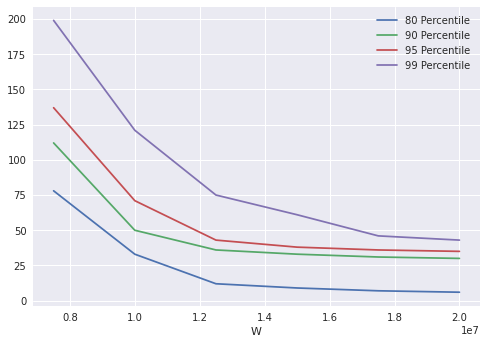
\includegraphics[width=\textwidth]{figures/e_coli-dbcm-error_percentiles-K31-D6}
        \caption{$d = 6$}\label{fig:ecoli-art-dbcm-errors-d6}
    \end{subfigure}%
    \begin{subfigure}{.5\textwidth}
        \centering
        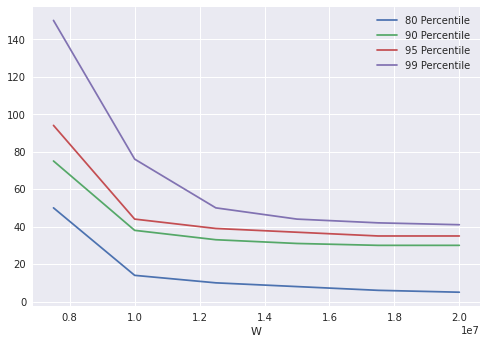
\includegraphics[width=\textwidth]{figures/e_coli-dbcm-error_percentiles-K31-D8}
        \caption{$d = 8$}\label{fig:ecoli-art-dbcm-errors-d8}
    \end{subfigure}
	\caption{\dBCM miscount percentiles as a function of $w$ for $d = 6$ and $d = 8$}\label{fig:ecoli-art-dbcm-errors}
\end{figure}

First, we observe that there is only a slight change for $w\geq 10\mega$ on both scenarios, but one could still argue that the errors can still be too high. However, we are not so much interested in the absolute counts per se, but rather as way of discerning real \kmers occurring in original sequence from spurious \kmers appearing only in the reads due to sequencing errors. In order to save memory, we would like to use the smallest values allowing for this separation.
To verify that the \dBCM can effectively differentiate between these two categories, we select the conservative values $w=10\mega$ and $d=6$ and compare the distribution of the count estimates with the actual values for the \kmer{s} in the reads. This comparison can be observed in Figure~\ref{fig:ecoli-art-dbcm-counts}. Note that, in the exact count distribution, close to $9\mega$ \kmer{s} have frequency between $2^4$ and $2^6$. This matches the expected number of real \kmer{s} from the sequence in forward and reverse complement forms. Although the estimated counts distribution is shifted right due to overcount, we see two peaks, one between $2^3$ and $2^4$, and the other between $2^6$ and $2^7$, indicating the high- and low-frequency categories may still be discernible although a threshold is not as clear as with the exact counts.
Combining these observations, we see that for $w \geq 10\mega$, $90\%$ of \kmer{s} have an error of no more than 50 regardless of $d$, such that we expect the majority of erroneous \kmer{s} to have an estimated count not much greater than that, while real \kmer{s} are expected to have a count not much lower than $80$ (the coverage). This suggests that high- and low-frequency \kmer{s} are likely to still be discernible based on a threshold in the 30--60 range.


\begin{figure}[htb]
    \centering
    \begin{subfigure}{.5\textwidth}
        \centering
        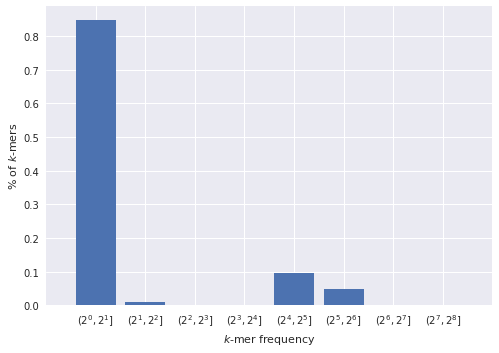
\includegraphics[width=\textwidth]{figures/e_coli-kmer_frequencies-exact-K31}
        \caption{Exact}\label{fig:ecoli-art-dbcm-counts-exact}
    \end{subfigure}%
    \begin{subfigure}{.5\textwidth}
        \centering
        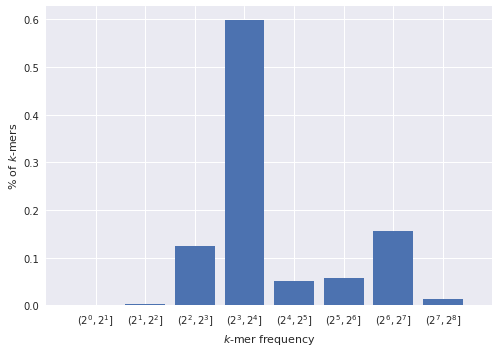
\includegraphics[width=\textwidth]{figures/e_coli-kmer_frequencies-estimated-K31-W10000000-D6}
        \caption{Estimated ($w = 10\mega, d = 6$)}\label{fig:ecoli-art-dbcm-counts-exact}
    \end{subfigure}
	\caption{\kmer count distribution}\label{fig:ecoli-art-dbcm-counts}
\end{figure}

Next we evaluate possible thresholds $t$ in the range $[1, 2c]$ by analyzing the \keyterm{true positive rate}, or \keyterm{sensitivity}, of the \dBCM, i.e. percentage of true \kmer{s} correctly identified, as well as its \keyterm{false positive rate}, i.e. percentage of false \kmer{s} erroneously identified as true, using each one of those values. The results are presented in Figure~\ref{fig:ecoli-art-dbcm-threshold-estimated}, where we can see that, without excluding any true \kmer{s} from the \dBG, we can filter out over $80\%$ of the spurious \kmer{s} from the reads by using $20 \leq t \leq 40$. However, comparing these results with the sensitivity and false positive rate if using the exact counts (Figure~\ref{fig:ecoli-art-dbcm-threshold-exact}), we can see that the number of false positives nearly doubles when keeping sensitivity maximized. In this dataset, this equates to nearly $9.7\mega$ spurious \kmer{s} being added to the \dBG, over $5\mega$ more than would be added using exact counts. In the following section we show that, despite this increase in number of spurious \kmer{s} represented in the \dBCM, only a fraction of them are reachable in traversal, such that this representation still succeeds in filtering out erroneous \kmer{s}.

A \dBCM with $w = 10\mega$ and $d = 6$ requires $16 \times 10\mega \times 6 = 960\mega$ bits, or $120$MB. The time needed for construction of the \dBCM is linear on the total number of bases in the reads, and took about $6$ minutes in our experimental environment.

\begin{figure}[htbp]
    \centering
    \begin{subfigure}{.5\textwidth}
        \centering
        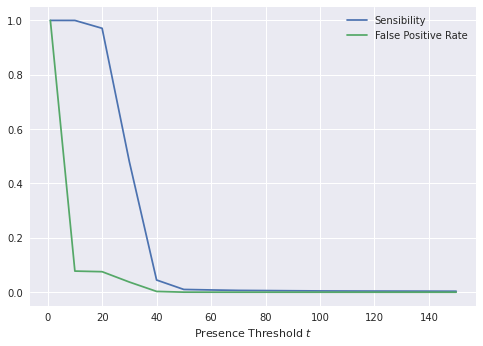
\includegraphics[width=\textwidth]{figures/e_coli-threshold_exploration-K31-exact}
        \caption{Exact counts}\label{fig:ecoli-art-dbcm-threshold-exact}
    \end{subfigure}%
    \begin{subfigure}{.5\textwidth}
        \centering
        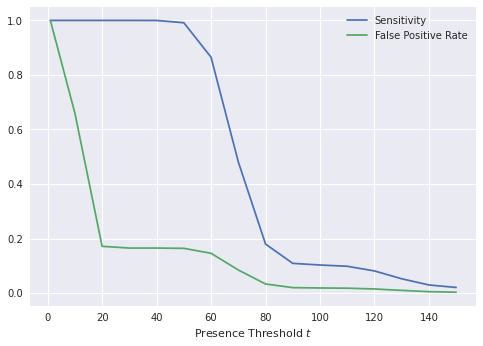
\includegraphics[width=\textwidth]{figures/e_coli-threshold_exploration-K31-W10000000-D6}
        \caption{Estimated by \dBCM ($w=10\mega, d=6$)}\label{fig:ecoli-art-dbcm-threshold-estimated}
    \end{subfigure}
    \caption{Sensitivity and False Positive Rate of a \dBCM with $w = 10\mega$ and $d = 6$ as a function of the presence threshold $t$}\label{fig:ecoli-art-dbcm-threshold}
\end{figure}

\section{Filtering through traversal}
\label{sec:results-dbcm-traversal}

As discussed in Section~\ref{sec:pipeline}, we expect many of the spurious \kmer{s} inserted into the \dBG due to overcoming the frequency threshold to be isolated from the main components of the graph, containing the real \kmer{s}. By traversing the graph from a small sample of these high-frequency \kmer{s}, we expect never to visit most of these disconnected components, such that using the set of \kmer{s} visited during a full traversal, rather than the set of high-frequency \kmer{s}, to construct a representation of the \dBG should lead to \remove{fewer distinct \kmer{s} inserted into the graph, allowing for} a more succinct representation.

To evaluate this hypothesis, we constructed a \dBCM with $w = 10\mega$, $d = 6$, and $t = 40$, from the unprocessed reads. We then traversed the graph from a subset of high-frequency \kmer{s} at the beginning of the reads\remove{, logging the \kmer{s} that were queried and their query results}. \change{Afterwards, we counted the number of queried \kmer{s} to be $\approx 9.62\mega$, as well as the number of those that were visited $\approx 9.58\mega$}{Approximately $9.62\mega$ \kmers were queried in the process, of which $\approx 9.58\mega$ were effectively visited}. Of those visited, only $173\kilo$ were not found in the original DNA sequence in either forward or reverse complement form, or approximately $1.8\%$ of the number of spurious \kmer{s} that would be added into a \dBG from the reads alone, based on the count estimated by the same \dBCM, and $3.8\%$ of the spurious \kmer{s} from the reads that would have been added based on their exact counts \change{}{(considering the same threshold)}. In a hashtable-based representation, such as the \dBHT, this would reduce the number of cells needed to represent the \dBG for this organism by \emph{one third} when compared with using the exact counts as the requirement for insertion.

% Traversing the \dBCM was done in around $30$ seconds when the queried \kmer{s} were not being logged to an output file, and twice that when writing to disk.\asq{Eu acho que esse resultado de tempo é meio inutilizável, porque eu usei um set em memória dos \kmer{s} visitados, de forma que isso não é escalável para genomas maiores. Não só a travessia, do jeito que está implementada agora, seria impossível sem uma quantidade enorme de memória, como ela acabaria usando uma representação não-sucinta do \dBG para ser capaz de dizer se um \kmer foi visitado ou não. Seria necessário fazer a travessia usando do disco, ou usar alguma outra estrutura sucinta através da qual pudessemos identificar quais \kmer{s} foram visitados. No final das contas talvez acabe não fazendo sentido? O mesmo vale para a travessia da dBHT}

\section{The \dBHT as a NDS}
\label{sec:results-dbht}

Finally, we want to evaluate how much different are the graphs represented by the \dBCM and the \dBHT generated from it. Note that, contrary to the \dBCM, any node inserted into the \dBHT found when queried, and likewise the outedges, such that there should be no loss in sensitivity when going from one representation to the other. However the \dBHT may introduce errors due to collisions, because the \kmer is not directly saved in the hashtable, but only its fingerprint. If two \kmer{s} with the same fingerprints are mapped to the same cell, we may take one for the other. This might lead to distinct \kmer{s} sharing the same set of outedges which, in turn, can result in false \kmer{s} being queried and incorrectly determined to be represented in the graph. The chance of collision, however, is controlled by the choice of load factor $\alpha$. Therefore, we evaluate the traversal performance of \dBHT{s} with varying load factors $\alpha \in \{0.5, 0.55, \ldots, 0.85, 0.9\}$, all constructed from the same \dBCM with $w = 10\mega$, $d = 6$, and $t = 40$.

In Figure~\ref{fig:ecoli-art-dbht-traversal-queryfound}, we can see that both the number of \kmer{s} queried during the traversal, and number of \kmer{s} actually visited, grow with $\alpha$, as the table size shrinks and collisions become more frequent. This  naturally results \change{in a growth of in the number of}{more} false positives, as evidenced in Figure~\ref{fig:ecoli-art-dbht-traversal-positives}. Note that, compared to the \dBCM, the false positive rate is about twice as high, even in the best case with $\alpha = 0.5$. However, even in the worst case, with $\alpha = 0.9$, the number of spurious \kmer{s} \remove{considered represented in the \dBG} is less than $40\%$ of what would be considered \paguso{from the reads???} based on \emph{exact} counts alone. These spurious \kmer{s} also represent only a small portion, $\approx 15\%$, of the the resulting graph.\asq{Eu queria trazer, aqui, uma comparação com os resultados obtidos por Pell \emph{et al.}, no qual eles mostram que uma taxa de falsos positivos (que eles definem como a chance de que um \kmer espúrio qualquer seja considerado representado no grafo) de 15\% não causa a conexão de \kmer{s} distantes. Sendo que 15\% de chance que um \kmer qualquer seja considerado presente no grafo significa que mais do que 15\% do grafo vão ser \kmer{s} espúrios (em um exemplo que eles dão com um grafo circular com 1000 \kmer{s}, se a gente assumisse que o grafo é perfeitinho, cada \kmer tem apenas um vizinho, então 3000 \kmer{s} espúrios são consultados, com a taxa em 15\% esperamos 450 deles sejam considerados representados, então 31\% do grafo, $450 / 1450$, seriam \kmer{s} espúrios, bem mais que nossos 15\%, e, ainda assim, o grafo não teria problema de \kmer{s} reais distantes serem conectados). Então eu acredito que daria pra mostrar que mesmo um $\alpha = 0.9$ ainda poderia ser usado pra montagem do genoma.} 
\paguso{Não entendi todos os detalhes do argumento, mas a questão é que se vc não tem os dados pra mostrar, acho que não vale a pena}
\change[Não precisa de um gráfico para mostrar uma constante]{Figure~\ref{fig:ecoli-art-dbht-traversal-sensitivity} confirms that there is no loss in sensitivity from going from the \dBCM representation to the \dBHT.}{Our experiments also do confirm that there is no sensitivity loss in going from the \dBCM to the \dBHT in the sense that all real \kmers are still queried and visited in the traversal in all tested scenarios.}\paguso{confirmar que é isso mesmo}

\begin{figure}[htbp]
    \centering
    \begin{subfigure}{.5\textwidth}
        \centering
        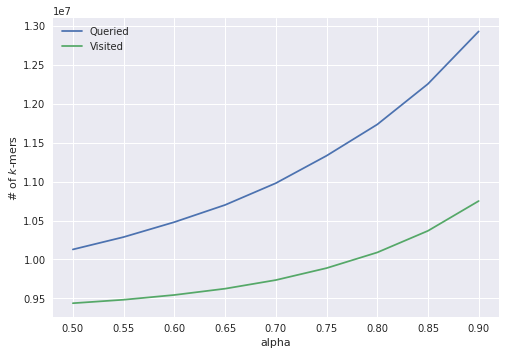
\includegraphics[width=\textwidth]{figures/e_coli-dbht-queried_and_found}
        \caption{Number of \kmer{s} queried (blue) and visited (green)}\label{fig:ecoli-art-dbht-traversal-queryfound}
    \end{subfigure}
    \begin{subfigure}{.5\textwidth}
        \centering
        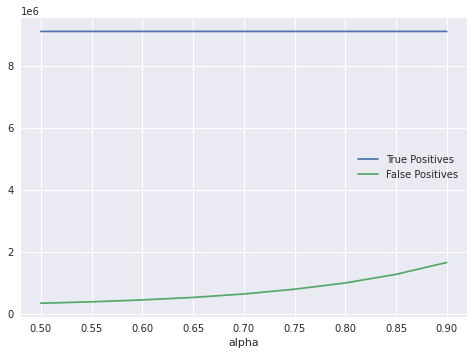
\includegraphics[width=\textwidth]{figures/e_coli-dbht-true_and_false_positive_counts}
        \caption{True (blue) and false (green) positive counts}\label{fig:ecoli-art-dbht-traversal-positives}
    \end{subfigure}%
\paguso{remover essa figura c porque ela não tem informação que a justifique.}
    \begin{subfigure}{.5\textwidth}
        \centering
        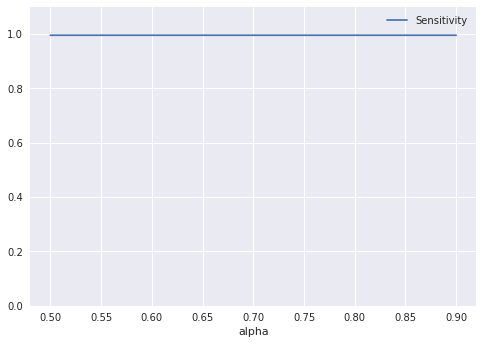
\includegraphics[width=\textwidth]{figures/e_coli-dbht-sensitivity}
        \caption{Sensitivity}\label{fig:ecoli-art-dbht-traversal-sensitivity}
    \end{subfigure}
    \caption{Traversal results for \dBHT according to load factor $\alpha$}\label{fig:ecoli-art-dbcm-threshold}
\end{figure}


\paguso{Realmente o tempo e memória estão fazendo falta. Você deu números exatos para o tamanho do \dBCM, então seria bom também dar por \dBHT para poder comparar. Ficou faltando uma justificativa para passar do DBCM para DBHT. Você mostrou que não piora, e até mencionou de forma geral que vc tem uma representação mais sucinta, mas não mostrou com números uma vantagem decisiva.}
